\documentclass[11pt,english]{article}
\usepackage[T1]{fontenc}

\usepackage{geometry}
\geometry{verbose,tmargin=2cm,bmargin=2cm,lmargin=3cm,rmargin=3cm}

\usepackage{fancyhdr}
\pagestyle{fancy}
\fancyhf{}
\rhead{OpenSHMEM Analzyer Guide}
\lhead{}
\cfoot{\thepage}

\usepackage[english]{babel}
\usepackage{graphicx}

\usepackage{fancybox}

\usepackage[unicode=true]{hyperref}

\usepackage[parfill]{parskip}

\usepackage[usenames,dvipsnames,svgnames,x11names]{xcolor}
\definecolor{ListingBG}{rgb}{0.91,0.91,0.91}

\usepackage{listings}
\lstset {
  basicstyle=\scriptsize\ttfamily,
  backgroundcolor=\color{ListingBG},
  keywordstyle=\color{blue}\textbf,
  frame=tlBR,
  language=C,
}

\newcommand{\HRule}{\rule{\linewidth}{0.5mm}}

\usepackage{xspace}
\newcommand{\openshmem}{\mbox{OpenSHMEM}\xspace}

\usepackage{alltt}


\begin{document}

\begin{titlepage}
  \begin{center}

    \vspace{1.0in} ~ \\

    \HRule \\[0.1in]
    {\LARGE \textsc{The OpenSHMEM Analyzer}} \\
    \vspace{0.2in}
    {\LARGE Version 1.0} \\
%    \vspace{0.2in}
%    {\LARGE DRAFT} \\
    \HRule \\[0.5in]

    \vspace{0.5in}

    Oak Ridge National Laboratory \\
    Computer Science Department and Mathematics Division \\
    Computer Science Research Group \\
    Extreme Scale Systems Center \\
    \vspace{0.1in}
    {\small \url{http://www.csm.ornl.gov/essc/}} \\

    \vspace{0.4in}

    University of Houston \\
    Computer Science Department \\
    High Performance Tools Group \\
    \vspace{0.1in}
    {\small \url{http://web.cs.uh.edu/~hpctools/}}

    \vspace{1.0in}

    \today

  \end{center}
\end{titlepage}


\tableofcontents
\listoffigures
\pagebreak

\section*{Preface}

This User's Manual describes the \openshmem Analyzer, a tool that
provides source code analysis and correctness checks capabilities to
the user. It provides a range of information about the source program
in textual or graphical format. The \openshmem Analyzer relies on web
browsers and the graph library GraphViz to render its graphs and use
of hyperlinks to navigate to the source code and warning messages.

\subsection*{Audience Description}

This manual is a user's guide only. Users are expected to have a basic
knowledge of the structure of programs and some experience with C and
\openshmem programming. The \openshmem Analyzer is available on Red Hat
/ SUSE systems with x86/x86-64 processors. It is assumed that users
are familiar with the basic commands on these systems.

\subsection*{Organization}

This User's Guide is structured into the following sections
% and appendices:

\begin{description}
\item[Section~\ref{chapter:introduction}:~\nameref{chapter:introduction}]
  gives an overview of the \openshmem Analyzer Tool and describes its
  major goals
\item[Section~\ref{chapter:basic-usage}:~\nameref{chapter:basic-usage}]
  describes naming conventions, generated files and how to visualize
  the graphs and traverse the source code.
\item[Section~\ref{chapter:features}:~\nameref{chapter:features}]
  describes the features for local and global analysis of \openshmem
  programs and how to interpret the information within the graphs.
\item [Section~\ref{chapter:future}:~\nameref{chapter:future}] a quick
  view of what is the on-going work of the \openshmem Analyzer and its
  future functionality
\end{description}


\section{Introduction}
\label{chapter:introduction}

In this chapter we give an overview of the overall features of the
\openshmem Analyzer and describe the structure of the system.

\subsection{Major Goals of the \openshmem Analyzer}

Whenever application software is developed or ported to \openshmem from
a new or an existing one, the source code must be carefully analyzed
in order to understand many details of the current implementation
while at the same time avoid common errors in \openshmem
applications. The \openshmem Analyzer is a tool to support an
application developer or code owner who wishes to understand more his
C application. It provides a range of information including the
structure of a source program in a graphical browseable form. The
current input languages for the \openshmem Analyzer are C/C++,
\openshmem API 1.0c.

\openshmem is a standard for SHMEM library implementations. Many SHMEM
libraries exist but they do not conform to a particular standard and
have similar but not identical APIs and behavior, which hinders
portability. However, significant user efforts are required to
parallelize serial codes with \openshmem or further analyze and
optimize the performance of \openshmem programs. The \openshmem
Analyzer, with its comprehensive intra and inter procedural analysis
information, can be an indispensable assistant for writing, analyzing
and optimizing \openshmem applications.  The \openshmem Analyzer has an
interactive component. It provides a graphical user interface using
HTML to display its graphical displays and for navigating the source
code and error messages within them.

The \openshmem Analyzer is an on-going research project developed at
Oak Ridge National Laboratories with funding from DOD. Its
functionality is based on the OpenUH compiler infrastructure, which is
maintained by the HPCTools Group at the University of
Houston. The \openshmem Analyzer is intended to be an open source tool
available for the \openshmem community.

\section{Basic Usage of the \openshmem Analyzer}
\label{chapter:basic-usage}

In this chapter the user will find

\begin{itemize}
\item Some hints on preparing programs for the \openshmem Analyzer
\item Invoking the \openshmem Analyzer for the first time
\item Naming/Graphical conventions
\item How to visualize the results or manipulate graphs
\end{itemize}

\subsection{Preparing Your Program for the \openshmem Analyzer}

The first step of preparing a program to be analyzed by the \openshmem
Analyzer is to compile it using the tool with a special set of
flags. The user is responsible for modifying the application's
makefiles, in order to reflect the compiler and flags setting
changes. Since the \openshmem Analyzer is based on OpenUH the
following are the main drivers/compilers:

\vspace{0.1in}

\begin{center}
  \begin{tabular}{|l | l |}
    \hline
    uhcc & C compiler \\
    \hline
    uhCC & C++ compiler (beta evaluation) \\
    \hline
  \end{tabular}
\end{center}

\vspace{0.1in}

In order to prepare your program, you must add the following flags:
-osa -O3 for the compile (-c) and link commands as follows.

\subsubsection*{Compile commands:}

\begin{lstlisting}[language=bash]
  $ uhcc -osa -O3 -c myfile.c
  $ uhcc -osa -O3 -c myfile2.c
\end{lstlisting}

\subsubsection*{Link command:}

\begin{lstlisting}[language=bash]
  $ uhcc -osa -O3 myfile.o myfile2.o -o myprogram 
\end{lstlisting}

Note: To avoid long compilation times, the less aggressive flag -O2
can be used.

In this example, the \openshmem Analyzer will generate a
series of files with extensions: html, gif, dot, map, msg.

\subsection{Using the \openshmem Analyzer}

There are two modes of visualizing the results of the \openshmem
Analyzer: at the command line or via a web browser. When you build
your program with the \openshmem Analyzer will display the warnings at
the command line. In addition, the \openshmem Analyzer is able to
display the warnings in a browser together with the program callgraph.

\subsubsection{Filename Conventions}

The \openshmem Analyzer creates several files with different extensions. 
The following command:

\begin{lstlisting}[language=bash]
  $ uhcc -osa -O2 myfile.c -o myprogram
\end{lstlisting}

will generate the following files:

\vspace{0.1in}

\begin{center}
  \begin{tabular}{| l | p{10cm} |}
    \hline
    myprogram.html & This is the .html file that can be open with a browser. It contains the callgraph and the warning messages from the tools \\
    \hline
    myprogram.msg & Contains the error messages collected during inter-procedural analysis phase \\
    \hline
    myfile.c.html & This will contain the HTML version of the source code with syntax highlighted and line number target links \\
    \hline
    myfile.c.msg & List of error messages generated during intra-procedural analysis phase \\
    \hline
    myprogram.dot & This file contains the callgraph of the application in the GraphViz format \\
    \hline
    myprogram.gif & This file contains the .gif image version of the callgraph \\
    \hline
  \end{tabular}
\end{center}

\subsection{How the \openshmem Analyzer works}

The \openshmem analyzer relies on intra-procedural and inter-procedural
analysis to detect potential semantic program errors in the
application. The types of warnings reported are displayed during the
different compilation phases of the tool. Figure~\ref{fig:phases} shows
how the different phases generate the different analyses:

\begin{figure}[!h]
  \begin{center}
    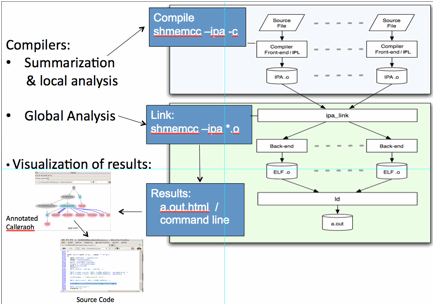
\includegraphics[width=0.5\textwidth]{./image002}
    \caption{Phases generating the different analyses}
    \label{fig:phases}
  \end{center}
\end{figure}

The \openshmem Analyzer generates warning messages at different
compilation stages of the code. The warning messages are then
displayed at command line or together in the callgraph.  The \openshmem
analyzer does not produce an executable file (in future releases this
feature will be enabled).

\section{Features of the \openshmem Analyzer}
\label{chapter:features}

\subsection{Overview}

The \openshmem Analyzer will generate an HTML file file with the
callgraph of a program that can be related to the source code via HTML
links. In addition the main HTML file contains a list of warning
messages generated by the tool and that can be related to the source
code via HTML links.

The following command opens the HTML file that contains the callgraph
and the error messages of the program (based on the previous example).

\begin{lstlisting}[language=bash]
  $ firefox myprogram.html
\end{lstlisting}

\subsubsection{Callgraph}

The call graph gives the structure of the program, where there is a
node for each procedure in the program and a directed edge links a
pair of nodes if and only if the procedure corresponding to the source
node may invoke the sink node's procedure at run time. If you click on
a node, the source text of the corresponding procedure will be
displayed in the HTML browser. The edges of the graph represent the
different callsites where the procedures are invoked. The user can
click on the edges to relate them to the source code. The callgraph
nodes are colored in the following format:

\vspace{0.1in}

\begin{center}
  \begin{tabular}{| p{10cm} | l |}
    \hline
    Procedures containing \openshmem calls & \textcolor{LightBlue}{light blue} \\
    \hline
    Procedures not containing \openshmem calls & \textcolor{Silver}{silver} \\
    \hline
    Procedures representing \openshmem & \textcolor{Pink}{pink} \\
    \hline
  \end{tabular}
\end{center}

\vspace{0.1in}

For the edges, callsites to \openshmem are colored:

\vspace{0.1in}

\begin{center}
  \begin{tabular}{| p{10cm} | l |}
    \hline
    I/O operations (i.e.\ puts, gets) & \textcolor{Blue}{blue} \\
    \hline
    Reductions & \textcolor{Purple}{purple} \\
    \hline
    Broadcasts & \textcolor{Red}{red} \\
    \hline
    Atomics & \textcolor{Orange}{orange} \\
    \hline
    Memory management calls (i.e.\ dynamic allocation / deallocation of symmetric memory) & \textcolor{Yellow}{yellow} \\
    \hline
    State calls (i.e.\ num\_pes, my\_pe) & \textcolor{Green}{green} \\
    \hline
    Synchronization calls & \textcolor{Red}{red} \\
    \hline
  \end{tabular}
\end{center}

\vspace{0.1in}

Figure~\ref{fig:is-callgraph} shows a portion of a callgraph generated
for the IS NAS Parallel Benchmark:

\begin{figure}[!h]
  \begin{center}
    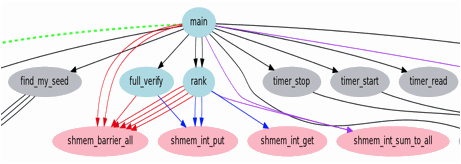
\includegraphics[width=0.8\textwidth]{./image004}
    \caption{The \openshmem callgraph of the IS NAS parallel benchmark}
    \label{fig:is-callgraph}
  \end{center}
\end{figure}

In addition to the callgraph, the color legend for the nodes and edges
is displayed in figure~\ref{fig:colors}

\vspace{0.1in}

\begin{figure}[!h]
  \begin{center}
    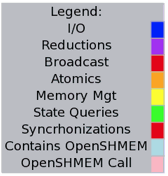
\includegraphics[width=0.25\textwidth]{./image006}
    \caption{The Color legend for the callgraph of an \openshmem program}
    \label{fig:colors}
  \end{center}
\end{figure}

When a node or a callsite is clicked, the browser will display the
corresponding source code with highlight syntax formatted in HTML, as
in figure~\ref{fig:app-source}.

\vspace{0.1in}

\begin{figure}[!h]
  \begin{center}
    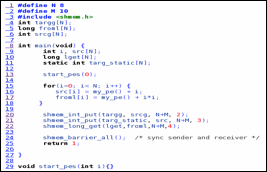
\includegraphics[width=0.6\textwidth]{./image008}
    \caption{Application source code as displayed in the browser}
    \label{fig:app-source}
  \end{center}
\end{figure}

\subsection{Displaying the \openshmem Analyzer Warnings}

The \openshmem Analyzer is able to display \openshmem warning messages
together with the callgraph. The warning messages are also displayed
when the tool is invoked at command line. When the warning messages
are displayed with the callgraph, each message contains an HTML link
that relates the message to the source. Figure~\ref{fig:warnings} is
an example of how the \openshmem Analyzer displays its warning messages
together with the source code.

\vspace{0.1in}

\begin{figure}[!h]
  \begin{center}
    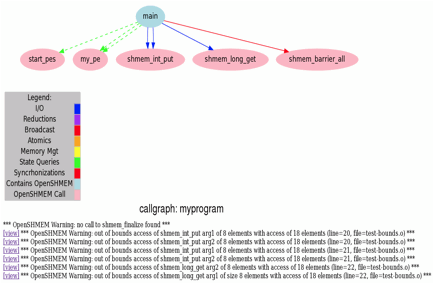
\includegraphics[width=1.0\textwidth]{./image010}
    \caption{Callgraph with the \openshmem Analyzer warning messages.
      The warning message contains a link to the source code}
    \label{fig:warnings}
  \end{center}
\end{figure}

The messages contain the line number and the source file name of the
\openshmem call that is triggering the warning.

\subsection{Analysis available in the \openshmem Analyzer}

The \openshmem Analyzer is able to perform the following analysis:

\vspace{0.1in}

\begin{itemize}
\item Check the ordering of \openshmem initialization and finalization
  calls.
\item Check if there is an \openshmem initialization call in the
  program.
\item Check if there are more than one \openshmem initialization call.
\item Check if \openshmem calls are using symmetric memory variables
\item Check if the \openshmem calls arguments are of the correct types
  or storage allocation for \openshmem typeless calls.
\item Check for out-of-bounds access for arrays in \openshmem calls.
\item Check for out-of-bounds strided access of arrays.
\item Check if one of the arguments of the \openshmem calls evaluates
  to NULL.
\item Perform constant propagation and common sub-expression
  elimination to simplify the arguments of an \openshmem call. This is
  useful to check if some arguments evaluate to constants or to
  simplify the analysis and accuracy of the tool.
\item Check if pointers to symmetric data are allocated with shmalloc
  calls
\item Check if any variables used in expression for pointer arithmetic
  of symmetric variables are initialized.
\item Check if global pointers to symmetric data are initialized.
\item Check if pointers to symmetric data are aliased with other
  pointers that can have side-effects to the \openshmem call.
\end{itemize}

\subsection{The \openshmem Analyzer Warnings messages}

The following shows a list of warning messages examples output by the tool

\subsubsection{Multiple \openshmem initialization call}

\begin{lstlisting}
  int main(...)  {                void sub (...) {
      ...                             ...
      start_pes();                    start_pes();       
      sub(...);                     } 
  }
\end{lstlisting}
\begin{alltt}
  *** \openshmem Warning: more than one \openshmem initialization call found ***
\end{alltt}

\subsubsection{Non-symmetric variable used in \openshmem call}

\begin{lstlisting}
  int sub(...) {
    long target, source;
    ...
    shmem_long_get(target, source, ...);
  }
\end{lstlisting}
\begin{alltt}
  *** \openshmem Warning: non-symmetric variable in arg2 of shmem_long_get 
  (line=65, file=badget.o) ***
\end{alltt}

\subsubsection{Out of bounds accesses in \openshmem call}

\begin{lstlisting}
  #define N 8
  #define M 8

  int sub (...) {
    ...
    static targ[N], src[N];
    ...
    shmem_int_put(targ, src, N + M, 2);
    ...
  }
\end{lstlisting}
\begin{alltt}
  *** \openshmem Warning: out of bounds access of shmem_int_put arg1 of 8 elements 
  with access of 16 elements (line=20, file=test-bounds.o) ***
\end{alltt}

\subsubsection{Out of bounds accesses in \openshmem call determined with constant propagation (must use -O3)}

\begin{lstlisting}
  #define N 8
  #define M 8

  int sub (...) {
    int len = N;
    static targ[N], src[N];
    ...
    for(i = 0; i < M; i++) len++;
    ...
    shmem_int_put(targ, src, len, 2);
    ...
  }     
\end{lstlisting}
\begin{alltt}
  *** \openshmem Warning: out of bounds access of shmem_int_put arg1 of 8 elements 
  with access of 16 elements (line=23, file=test-bounds-constprog.o) ***
\end{alltt}

\subsubsection{Out of bounds accesses in \openshmem call with strided access}

\begin{lstlisting}
  int src2[N];
  ...
  int sub(...) {
    ...
    shmem_iget32(dest2, src2, 1, 2, N, npes - 1);
    ...
  }
\end{lstlisting}
\begin{alltt}
  *** \openshmem Warning: out of bounds access of shmem_iget32 arg2 of 7 elements 
  with access of 14 elements (line=297, file=test_shmem_get_globals.o) ***
\end{alltt}

\subsubsection{Pointer is not initialized with the wrong memory allocator (non-symmetric)}

\begin{lstlisting}
  int sub(...) {
    ...
    float *y;
    ...
    y = (float *) malloc((n_local1 - n_local0 + 2) * sizeof(float));
    ...
    shmem_float_put(&y[n_local0-1+1], &y[n_local1-1], 1, _my_pe() + 1);
    ...
  } 
\end{lstlisting}
\begin{alltt}
  *** \openshmem Warning: variable arg1 of call shmem_float_put is initialized with 
  malloc, line=35, file=shmem\_heap.o) ***
\end{alltt}

\subsubsection{Global Pointer is not initialized}

\begin{lstlisting}
  float *y;

  int sub(...) {
    ...
    shmem_float_put(&y[n_local0-1+1], &y[n_local1-1], 1, _my_pe() + 1);
    ...
  }
\end{lstlisting}
\begin{alltt}
  *** \openshmem Warning: global variable arg1 of call shmem_float_put is 
  uninitialized line=20, file=shmem_heap-global.o) ***
\end{alltt}

\subsubsection{Wrong storage type for typeless \openshmem call}

\begin{lstlisting}
  long lfrom;

  int sub(void) {
    ...
    shmem_get32(lget, froml, N, 4);
    ...
  }
\end{lstlisting}
\begin{alltt}
  *** \openshmem Warning: wrong storage class of shmem_get32 arg2 of 8 bytes 
  (line=23, file=test-types.o) ***
\end{alltt}

\subsubsection{Symmetric variable in the \openshmem call may be aliased with a pointer}

\begin{lstlisting}
  int sub(...) {
    ...
  }
\end{lstlisting}
\begin{alltt}
  *** \openshmem Warning: Symmetric Variable named y in arg1 of \openshmem call 
  (line=37, file=1_put_afteruse_g.c) may be aliased with the pointer in line 37***
\end{alltt}

\section{Ongoing and Future Work}
\label{chapter:future}

We plan to develop a stand-alone user interface to present an
interactive callgraph and control flow graph that are aware of
\openshmem calls and develop a triage between these different views.
The idea is that there will be a data flow view that originates from
\openshmem calls and enables the user to see the use-define chains that
can help to keep track of the use and definition of pointers in
\openshmem calls. This will help the user evaluate the placement of a
particular call and how it is related to the rest of the application
more intuitively.  In addition, we could develop a view to see how
symmetric variables are accessed in the entire application, since
symmetric variables can affect many procedures (e.g.\ global variables,
interprocedural pointers). These sorts of views are important to
understand the overall side effects of the application.

The \openshmem Analyzer is moving toward a proper infrastructure to
perform parallel data flow analysis is needed, and apply the
state-of-the-art and how this relates to the context of \openshmem. As
a first step, we will explore the concept of program slicing at the
process level, which is the process for separating the different
control flow graphs from different processes. The idea is to simplify
the control flow graphs of a program per process and correctly denote
synchronizations across them. Through graph analysis we can classify
the different process control-flowgraphs into subsets that can be used
to represent optimizations and where classical program optimizations
can be applied per SHMEM task.

We plan to explore how to integrate better the \openshmem Analyzer to
the \openshmem library in a way that is more compiler friendly. We need
to make sure the library implementation allows the compiler to analyze
it and optimize it together with the application. This will include
the inlining of all \openshmem calls, their specialization to the
application context, constant propagation/dead code elimination, and
elimination of redundant runtime checks. The \openshmem Analyzer could
perform checks at compile time and define a set of assertions that we
can enforce at runtime to make sure the library is run in the right
context, reducing runtime checks and overheads.

We will also explore how to integrate dynamic information to the
\openshmem Analyzer. This will mean integrating it with performance
tools such as TAU and the \openshmem Tracer. We will combine the
\openshmem Analyzer instrumentation with the \openshmem wrappers of
these tools to gather calculate frequently executed paths in the
control graph and callgraph or values of variables at a given point of
execution. This will help toward feedback and present to the user a
dynamic callgraph and control flow graph, that shows the execution
code coverage and the frequently accessed code path that can be
specialized.

\end{document}
